% This is auto-generated file: do not edit!
% Exported from microMathematics Plus, version 2.16


Este exemplo demonstra como preparar e
ajustar uma representação gráfica de
uma função. Por exemplo, queremos
desenhar tês funções diferentes:
\begin{center}\begin{tabular}{c}
  $f(x) := 25 + 10 \cdot sin \left( \sqrt{ \left| x \right| } \right) $
\end{tabular}\end{center}
\begin{center}\begin{tabular}{c}
  $g(x) := \frac{2}{{e}^{ \left| x \right|  / 15}} \cdot f \left( x \cdot 50\right) $
\end{tabular}\end{center}
\begin{center}\begin{tabular}{c}
  $h(x) := min \left( f \left( x\right) ,\, g \left( x\right) \right) $
\end{tabular}\end{center}

O argumento da função que representa os
valores-x serão tomados para N pontos
no intervalo [x1, x2]:
\begin{center}\begin{tabular}{ccc}
  $N := 300$ &
  $x1 := -30$ &
  $x2 := 30$ \cr
\end{tabular}\end{center}
\begin{center}\begin{tabular}{c}
  $x := \left[ x1,\, x1 + \left( x2 - x1 \right) / N \,..\, x2 \right]$
\end{tabular}\end{center}

Após as funções e seus argumentos forem
definidos, você pode adicionar a caixa
para desenhar usando o botão ''Novo
elemento'' na barra de ações ou o botão
''Adicionar desenho de função'' a partir
da barra de ferramentas:
\begin{center}\begin{tabular}{c} 
\includegraphics[resolution=320]{graphics/function_plot_fig1.png} \end{tabular}\end{center}
\begin{center}\begin{tabular}{c} 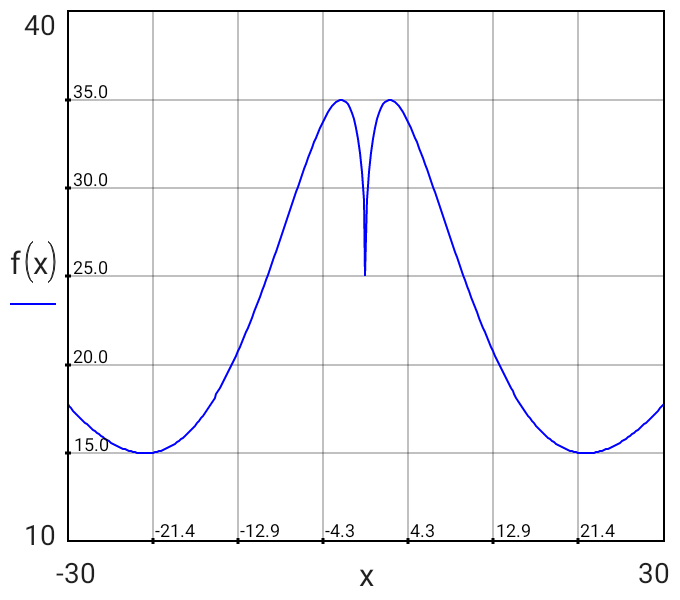
\includegraphics[resolution=320]{graphics/function_plot_fig2.png} \end{tabular}\end{center}

A função a ser desenhada será posta no
campo central-esquerdo. Também pode
ser uma função embutida ou declarada
previamente como uma expressão
matemática que contém qualquer outros
operadores e funções.

A função esntrada, que representa os
valores-x que serão postos no campo
central-esquerdo. Pode ser uma
variável do tipo intervalo ou uma
expressão matemática que contém uma
variável de intervalo.

Os outros quatro campos descrevem os
limites do desenho. Se estes elementos
premanecerem vazios, o programa
calculará valores correspondentes
automaticamente. Entretanto, você pode
editar estes campos a qualquer momento
e colocar lá os valores que sedejar.

Você pode desenhar diversas funções na
mesma visualização. Para adicionar uma
outra função, selecione a função
(segurando no campo central-esquerdo)
depois qual outra função deve ser
adicionada e toque no botão ''Adicionar
novo argumento'' a partir da barra de
tarefas:
\begin{center}\begin{tabular}{c} 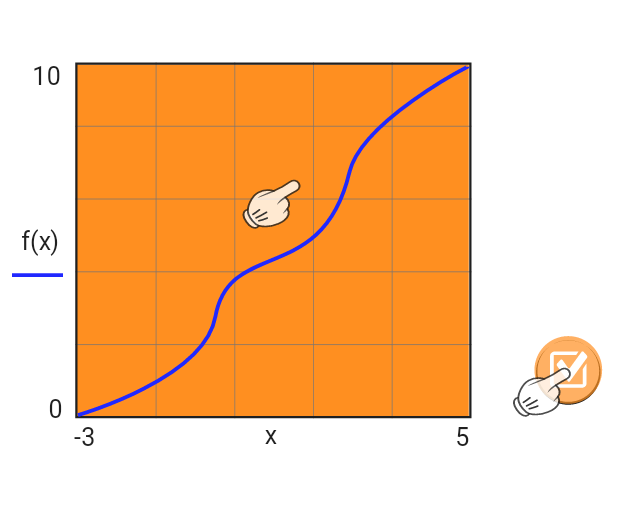
\includegraphics[resolution=320]{graphics/function_plot_fig3.png} \end{tabular}\end{center}
\begin{center}\begin{tabular}{c} 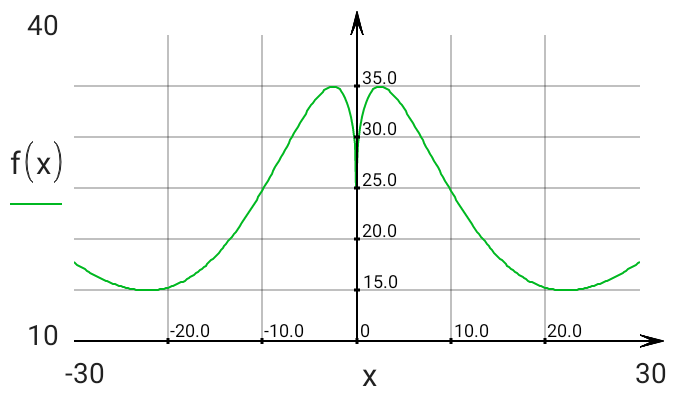
\includegraphics[resolution=320]{graphics/function_plot_fig4.png} \end{tabular}\end{center}

Segurando no centro da área de desenho,
o menu de contexto e o botão flutuante
''Propriedades do objeto'' aparecerá.
\begin{center}\begin{tabular}{c} 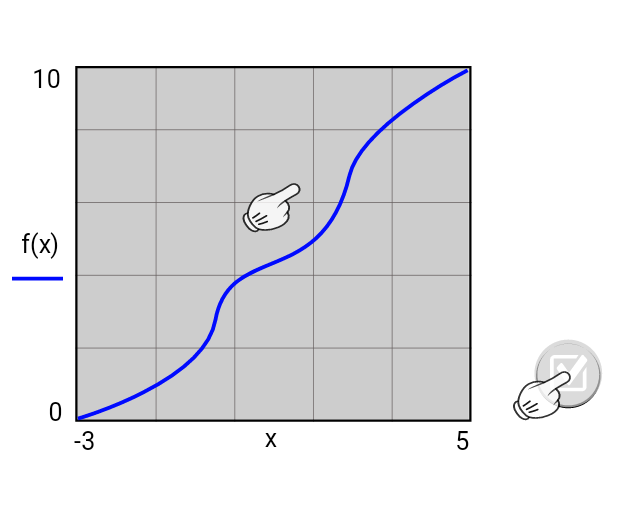
\includegraphics[resolution=320]{graphics/function_plot_fig5.png} \end{tabular}\end{center}

Se você tocar no botão flutuante, a
janela de ''Configurações de traço''
será exibida. Aqui, você pode alterar
o tamanho e aparência da área de
desenho. Por exemplo, o gráfico
cruzado parece assim:
\begin{center}\begin{tabular}{c} 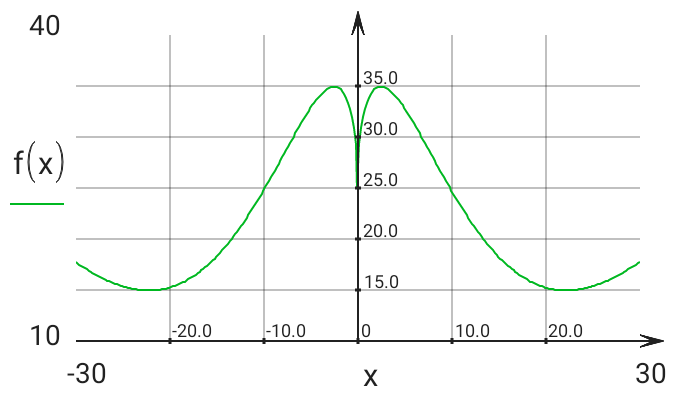
\includegraphics[resolution=320]{graphics/function_plot_fig6.png} \end{tabular}\end{center}

Você também pode alterar a cor da linha
de desenho, largura e aparência na
janela ''Configurações da linha''. Ela
aparece ao segurar no marcador de
linha abaixo do nome da função na área
esquerda do desenho:
\begin{center}\begin{tabular}{c} 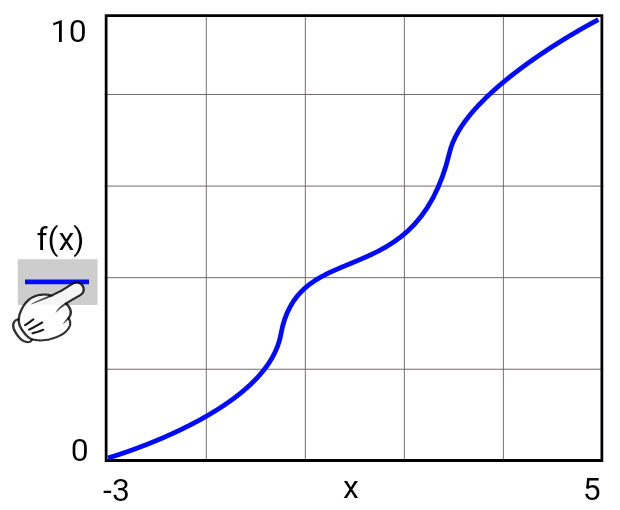
\includegraphics[resolution=320]{graphics/function_plot_fig7.png} \end{tabular}\end{center}

For example, we can use dotted lines:
\begin{center}\begin{tabular}{c} 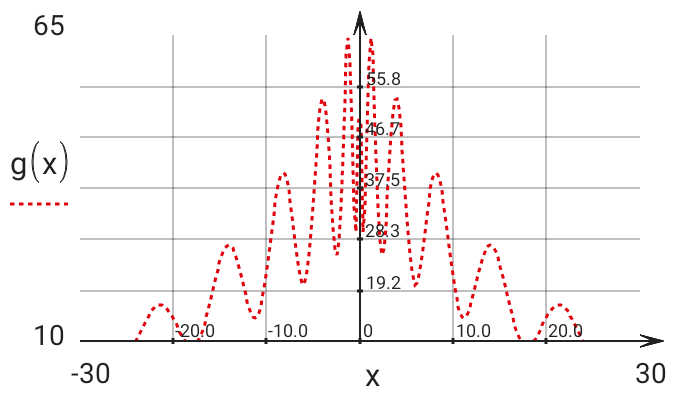
\includegraphics[resolution=320]{graphics/function_plot_fig8.png} \end{tabular}\end{center}

O número de eixos e rótulos e cor das
linahs de grade podem ser alteradas na
janela ''Configurações de grade''. Ela
aparece segurando na área livre entre
o valor mínimo de x (-30) e o símbolo
de argumento (x) ou entre o símbolo x
e o valor máximo de x (30) abaixo da
área de desenho:
\begin{center}\begin{tabular}{c} 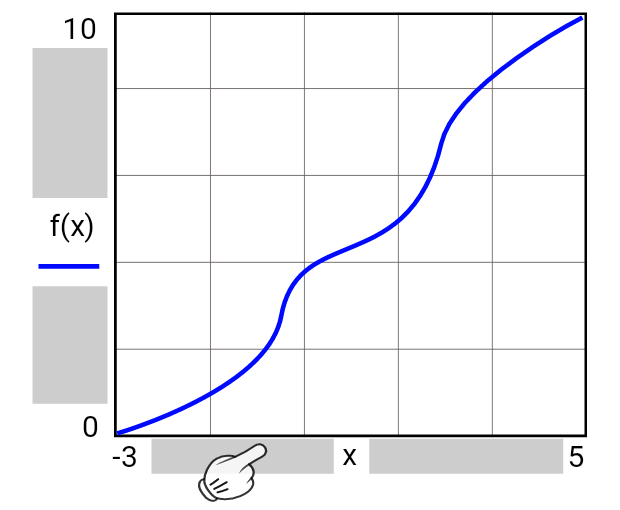
\includegraphics[resolution=320]{graphics/function_plot_fig9.png} \end{tabular}\end{center}
\begin{center}\begin{tabular}{c} 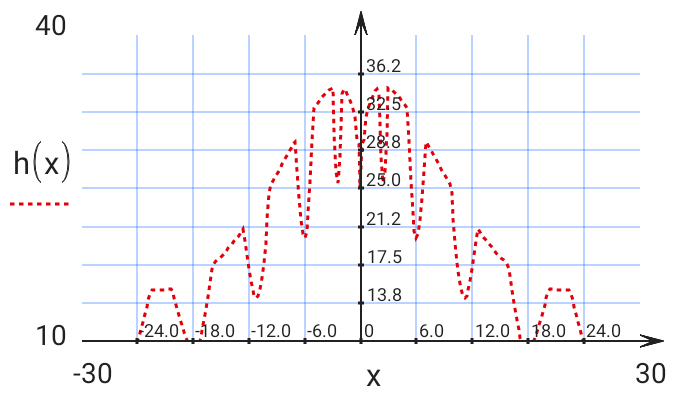
\includegraphics[resolution=320]{graphics/function_plot_fig10.png} \end{tabular}\end{center}

Para esconder a grade completamente
apenas defina o número de linhas da
grade para zero nos eixos vertical e
horizontal.